
%% bare_adv.tex
%% V1.4b
%% 2015/08/26
%% by Michael Shell
%% See: 
%% http://www.michaelshell.org/
%% for current contact information.
%%
%% This is a skeleton file demonstrating the advanced use of IEEEtran.cls
%% (requires IEEEtran.cls version 1.8b or later) with an IEEE Computer
%% Society journal paper.
%%
%% Support sites:
%% http://www.michaelshell.org/tex/ieeetran/
%% http://www.ctan.org/pkg/ieeetran
%% and
%% http://www.ieee.org/

%%*************************************************************************
%% Legal Notice:
%% This code is offered as-is without any warranty either expressed or
%% implied; without even the implied warranty of MERCHANTABILITY or
%% FITNESS FOR A PARTICULAR PURPOSE! 
%% User assumes all risk.
%% In no event shall the IEEE or any contributor to this code be liable for
%% any damages or losses, including, but not limited to, incidental,
%% consequential, or any other damages, resulting from the use or misuse
%% of any information contained here.
%%
%% All comments are the opinions of their respective authors and are not
%% necessarily endorsed by the IEEE.
%%
%% This work is distributed under the LaTeX Project Public License (LPPL)
%% ( http://www.latex-project.org/ ) version 1.3, and may be freely used,
%% distributed and modified. A copy of the LPPL, version 1.3, is included
%% in the base LaTeX documentation of all distributions of LaTeX released
%% 2003/12/01 or later.
%% Retain all contribution notices and credits.
%% ** Modified files should be clearly indicated as such, including  **
%% ** renaming them and changing author support contact information. **
%%*************************************************************************


% *** Authors should verify (and, if needed, correct) their LaTeX system  ***
% *** with the testflow diagnostic prior to trusting their LaTeX platform ***
% *** with production work. The IEEE's font choices and paper sizes can   ***
% *** trigger bugs that do not appear when using other class files.       ***                          ***
% The testflow support page is at:
% http://www.michaelshell.org/tex/testflow/


% IEEEtran V1.7 and later provides for these CLASSINPUT macros to allow the
% user to reprogram some IEEEtran.cls defaults if needed. These settings
% override the internal defaults of IEEEtran.cls regardless of which class
% options are used. Do not use these unless you have good reason to do so as
% they can result in nonIEEE compliant documents. User beware. ;)
%
%\newcommand{\CLASSINPUTbaselinestretch}{1.0} % baselinestretch
%\newcommand{\CLASSINPUTinnersidemargin}{1in} % inner side margin
%\newcommand{\CLASSINPUToutersidemargin}{1in} % outer side margin
%\newcommand{\CLASSINPUTtoptextmargin}{1in}   % top text margin
%\newcommand{\CLASSINPUTbottomtextmargin}{1in}% bottom text margin




%
\documentclass[10pt,journal]{IEEEtran}
% If IEEEtran.cls has not been installed into the LaTeX system files,
% manually specify the path to it like:
% \documentclass[10pt,journal,compsoc]{../sty/IEEEtran}


% For Computer Society journals, IEEEtran defaults to the use of 
% Palatino/Palladio as is done in IEEE Computer Society journals.
% To go back to Times Roman, you can use this code:
%\renewcommand{\rmdefault}{ptm}\selectfont





% Some very useful LaTeX packages include:
% (uncomment the ones you want to load)



% *** MISC UTILITY PACKAGES ***
%
%\usepackage{ifpdf}
% Heiko Oberdiek's ifpdf.sty is very useful if you need conditional
% compilation based on whether the output is pdf or dvi.
% usage:
% \ifpdf
%   % pdf code
% \else
%   % dvi code
% \fi
% The latest version of ifpdf.sty can be obtained from:
% http://www.ctan.org/pkg/ifpdf
% Also, note that IEEEtran.cls V1.7 and later provides a builtin
% \ifCLASSINFOpdf conditional that works the same way.
% When switching from latex to pdflatex and vice-versa, the compiler may
% have to be run twice to clear warning/error messages.
\usepackage{algorithmic}
\usepackage{amsmath}
\usepackage{textcomp}
\usepackage{graphicx}
\usepackage{listings}
  \usepackage{caption2}
% *** CITATION PACKAGES ***
%
\ifCLASSOPTIONcompsoc
  % The IEEE Computer Society needs nocompress option
  % requires cite.sty v4.0 or later (November 2003)
  \usepackage[nocompress]{cite}
\else
  % normal IEEE
  \usepackage{cite}
\fi
% cite.sty was written by Donald Arseneau
% V1.6 and later of IEEEtran pre-defines the format of the cite.sty package
% \cite{} output to follow that of the IEEE. Loading the cite package will
% result in citation numbers being automatically sorted and properly
% "compressed/ranged". e.g., [1], [9], [2], [7], [5], [6] without using
% cite.sty will become [1], [2], [5]--[7], [9] using cite.sty. cite.sty's
% \cite will automatically add leading space, if needed. Use cite.sty's
% noadjust option (cite.sty V3.8 and later) if you want to turn this off
% such as if a citation ever needs to be enclosed in parenthesis.
% cite.sty is already installed on most LaTeX systems. Be sure and use
% version 5.0 (2009-03-20) and later if using hyperref.sty.
% The latest version can be obtained at:
% http://www.ctan.org/pkg/cite
% The documentation is contained in the cite.sty file itself.
%
% Note that some packages require special options to format as the Computer
% Society requires. In particular, Computer Society  papers do not use
% compressed citation ranges as is done in typical IEEE papers
% (e.g., [1]-[4]). Instead, they list every citation separately in order
% (e.g., [1], [2], [3], [4]). To get the latter we need to load the cite
% package with the nocompress option which is supported by cite.sty v4.0
% and later.





% *** GRAPHICS RELATED PACKAGES ***
%
\ifCLASSINFOpdf
  % \usepackage[pdftex]{graphicx}
  % declare the path(s) where your graphic files are
  % \graphicspath{{../pdf/}{../jpeg/}}
  % and their extensions so you won't have to specify these with
  % every instance of \includegraphics
  % \DeclareGraphicsExtensions{.pdf,.jpeg,.png}
\else
  % or other class option (dvipsone, dvipdf, if not using dvips). graphicx
  % will default to the driver specified in the system graphics.cfg if no
  % driver is specified.
  % \usepackage[dvips]{graphicx}
  % declare the path(s) where your graphic files are
  % \graphicspath{{../eps/}}
  % and their extensions so you won't have to specify these with
  % every instance of \includegraphics
  % \DeclareGraphicsExtensions{.eps}
\fi
% graphicx was written by David Carlisle and Sebastian Rahtz. It is
% required if you want graphics, photos, etc. graphicx.sty is already
% installed on most LaTeX systems. The latest version and documentation
% can be obtained at: 
% http://www.ctan.org/pkg/graphicx
% Another good source of documentation is "Using Imported Graphics in
% LaTeX2e" by Keith Reckdahl which can be found at:
% http://www.ctan.org/pkg/epslatex
%
% latex, and pdflatex in dvi mode, support graphics in encapsulated
% postscript (.eps) format. pdflatex in pdf mode supports graphics
% in .pdf, .jpeg, .png and .mps (metapost) formats. Users should ensure
% that all non-photo figures use a vector format (.eps, .pdf, .mps) and
% not a bitmapped formats (.jpeg, .png). The IEEE frowns on bitmapped formats
% which can result in "jaggedy"/blurry rendering of lines and letters as
% well as large increases in file sizes.
%
% You can find documentation about the pdfTeX application at:
% http://www.tug.org/applications/pdftex





% *** MATH PACKAGES ***
%
%\usepackage{amsmath}
% A popular package from the American Mathematical Society that provides
% many useful and powerful commands for dealing with mathematics.
%
% Note that the amsmath package sets \interdisplaylinepenalty to 10000
% thus preventing page breaks from occurring within multiline equations. Use:
%\interdisplaylinepenalty=2500
% after loading amsmath to restore such page breaks as IEEEtran.cls normally
% does. amsmath.sty is already installed on most LaTeX systems. The latest
% version and documentation can be obtained at:
% http://www.ctan.org/pkg/amsmath





% *** SPECIALIZED LIST PACKAGES ***
%\usepackage{acronym}
% acronym.sty was written by Tobias Oetiker. This package provides tools for
% managing documents with large numbers of acronyms. (You don't *have* to
% use this package - unless you have a lot of acronyms, you may feel that
% such package management of them is bit of an overkill.)
% Do note that the acronym environment (which lists acronyms) will have a
% problem when used under IEEEtran.cls because acronym.sty relies on the
% description list environment - which IEEEtran.cls has customized for
% producing IEEE style lists. A workaround is to declared the longest
% label width via the IEEEtran.cls \IEEEiedlistdecl global control:
%
% \renewcommand{\IEEEiedlistdecl}{\IEEEsetlabelwidth{SONET}}
% \begin{acronym}
%
% \end{acronym}
% \renewcommand{\IEEEiedlistdecl}{\relax}% remember to reset \IEEEiedlistdecl
%
% instead of using the acronym environment's optional argument.
% The latest version and documentation can be obtained at:
% http://www.ctan.org/pkg/acronym


%\usepackage{algorithmic}
% algorithmic.sty was written by Peter Williams and Rogerio Brito.
% This package provides an algorithmic environment fo describing algorithms.
% You can use the algorithmic environment in-text or within a figure
% environment to provide for a floating algorithm. Do NOT use the algorithm
% floating environment provided by algorithm.sty (by the same authors) or
% algorithm2e.sty (by Christophe Fiorio) as the IEEE does not use dedicated
% algorithm float types and packages that provide these will not provide
% correct IEEE style captions. The latest version and documentation of
% algorithmic.sty can be obtained at:
% http://www.ctan.org/pkg/algorithms
% Also of interest may be the (relatively newer and more customizable)
% algorithmicx.sty package by Szasz Janos:
% http://www.ctan.org/pkg/algorithmicx




% *** ALIGNMENT PACKAGES ***
%
%\usepackage{array}
% Frank Mittelbach's and David Carlisle's array.sty patches and improves
% the standard LaTeX2e array and tabular environments to provide better
% appearance and additional user controls. As the default LaTeX2e table
% generation code is lacking to the point of almost being broken with
% respect to the quality of the end results, all users are strongly
% advised to use an enhanced (at the very least that provided by array.sty)
% set of table tools. array.sty is already installed on most systems. The
% latest version and documentation can be obtained at:
% http://www.ctan.org/pkg/array


%\usepackage{mdwmath}
%\usepackage{mdwtab}
% Also highly recommended is Mark Wooding's extremely powerful MDW tools,
% especially mdwmath.sty and mdwtab.sty which are used to format equations
% and tables, respectively. The MDWtools set is already installed on most
% LaTeX systems. The lastest version and documentation is available at:
% http://www.ctan.org/pkg/mdwtools


% IEEEtran contains the IEEEeqnarray family of commands that can be used to
% generate multiline equations as well as matrices, tables, etc., of high
% quality.


%\usepackage{eqparbox}
% Also of notable interest is Scott Pakin's eqparbox package for creating
% (automatically sized) equal width boxes - aka "natural width parboxes".
% Available at:
% http://www.ctan.org/pkg/eqparbox




% *** SUBFIGURE PACKAGES ***
%\ifCLASSOPTIONcompsoc
%  \usepackage[caption=false,font=footnotesize,labelfont=sf,textfont=sf]{subfig}
%\else
%  \usepackage[caption=false,font=footnotesize]{subfig}
%\fi
% subfig.sty, written by Steven Douglas Cochran, is the modern replacement
% for subfigure.sty, the latter of which is no longer maintained and is
% incompatible with some LaTeX packages including fixltx2e. However,
% subfig.sty requires and automatically loads Axel Sommerfeldt's caption.sty
% which will override IEEEtran.cls' handling of captions and this will result
% in non-IEEE style figure/table captions. To prevent this problem, be sure
% and invoke subfig.sty's "caption=false" package option (available since
% subfig.sty version 1.3, 2005/06/28) as this is will preserve IEEEtran.cls
% handling of captions.
% Note that the Computer Society format requires a sans serif font rather
% than the serif font used in traditional IEEE formatting and thus the need
% to invoke different subfig.sty package options depending on whether
% compsoc mode has been enabled.
%
% The latest version and documentation of subfig.sty can be obtained at:
% http://www.ctan.org/pkg/subfig




% *** FLOAT PACKAGES ***
%
%\usepackage{fixltx2e}
% fixltx2e, the successor to the earlier fix2col.sty, was written by
% Frank Mittelbach and David Carlisle. This package corrects a few problems
% in the LaTeX2e kernel, the most notable of which is that in current
% LaTeX2e releases, the ordering of single and double column floats is not
% guaranteed to be preserved. Thus, an unpatched LaTeX2e can allow a
% single column figure to be placed prior to an earlier double column
% figure.
% Be aware that LaTeX2e kernels dated 2015 and later have fixltx2e.sty's
% corrections already built into the system in which case a warning will
% be issued if an attempt is made to load fixltx2e.sty as it is no longer
% needed.
% The latest version and documentation can be found at:
% http://www.ctan.org/pkg/fixltx2e


%\usepackage{stfloats}
% stfloats.sty was written by Sigitas Tolusis. This package gives LaTeX2e
% the ability to do double column floats at the bottom of the page as well
% as the top. (e.g., "\begin{figure*}[!b]" is not normally possible in
% LaTeX2e). It also provides a command:
%\fnbelowfloat
% to enable the placement of footnotes below bottom floats (the standard
% LaTeX2e kernel puts them above bottom floats). This is an invasive package
% which rewrites many portions of the LaTeX2e float routines. It may not work
% with other packages that modify the LaTeX2e float routines. The latest
% version and documentation can be obtained at:
% http://www.ctan.org/pkg/stfloats
% Do not use the stfloats baselinefloat ability as the IEEE does not allow
% \baselineskip to stretch. Authors submitting work to the IEEE should note
% that the IEEE rarely uses double column equations and that authors should try
% to avoid such use. Do not be tempted to use the cuted.sty or midfloat.sty
% packages (also by Sigitas Tolusis) as the IEEE does not format its papers in
% such ways.
% Do not attempt to use stfloats with fixltx2e as they are incompatible.
% Instead, use Morten Hogholm'a dblfloatfix which combines the features
% of both fixltx2e and stfloats:
%
% \usepackage{dblfloatfix}
% The latest version can be found at:
% http://www.ctan.org/pkg/dblfloatfix


%\ifCLASSOPTIONcaptionsoff
%  \usepackage[nomarkers]{endfloat}
% \let\MYoriglatexcaption\caption
% \renewcommand{\caption}[2][\relax]{\MYoriglatexcaption[#2]{#2}}
%\fi
% endfloat.sty was written by James Darrell McCauley, Jeff Goldberg and 
% Axel Sommerfeldt. This package may be useful when used in conjunction with 
% IEEEtran.cls'  captionsoff option. Some IEEE journals/societies require that
% submissions have lists of figures/tables at the end of the paper and that
% figures/tables without any captions are placed on a page by themselves at
% the end of the document. If needed, the draftcls IEEEtran class option or
% \CLASSINPUTbaselinestretch interface can be used to increase the line
% spacing as well. Be sure and use the nomarkers option of endfloat to
% prevent endfloat from "marking" where the figures would have been placed
% in the text. The two hack lines of code above are a slight modification of
% that suggested by in the endfloat docs (section 8.4.1) to ensure that
% the full captions always appear in the list of figures/tables - even if
% the user used the short optional argument of \caption[]{}.
% IEEE papers do not typically make use of \caption[]'s optional argument,
% so this should not be an issue. A similar trick can be used to disable
% captions of packages such as subfig.sty that lack options to turn off
% the subcaptions:
% For subfig.sty:
% \let\MYorigsubfloat\subfloat
% \renewcommand{\subfloat}[2][\relax]{\MYorigsubfloat[]{#2}}
% However, the above trick will not work if both optional arguments of
% the \subfloat command are used. Furthermore, there needs to be a
% description of each subfigure *somewhere* and endfloat does not add
% subfigure captions to its list of figures. Thus, the best approach is to
% avoid the use of subfigure captions (many IEEE journals avoid them anyway)
% and instead reference/explain all the subfigures within the main caption.
% The latest version of endfloat.sty and its documentation can obtained at:
% http://www.ctan.org/pkg/endfloat
%
% The IEEEtran \ifCLASSOPTIONcaptionsoff conditional can also be used
% later in the document, say, to conditionally put the References on a 
% page by themselves.





% *** PDF, URL AND HYPERLINK PACKAGES ***
%
%\usepackage{url}
% url.sty was written by Donald Arseneau. It provides better support for
% handling and breaking URLs. url.sty is already installed on most LaTeX
% systems. The latest version and documentation can be obtained at:
% http://www.ctan.org/pkg/url
% Basically, \url{my_url_here}.


% NOTE: PDF thumbnail features are not required in IEEE papers
%       and their use requires extra complexity and work.
%\ifCLASSINFOpdf
%  \usepackage[pdftex]{thumbpdf}
%\else
%  \usepackage[dvips]{thumbpdf}
%\fi
% thumbpdf.sty and its companion Perl utility were written by Heiko Oberdiek.
% It allows the user a way to produce PDF documents that contain fancy
% thumbnail images of each of the pages (which tools like acrobat reader can
% utilize). This is possible even when using dvi->ps->pdf workflow if the
% correct thumbpdf driver options are used. thumbpdf.sty incorporates the
% file containing the PDF thumbnail information (filename.tpm is used with
% dvips, filename.tpt is used with pdftex, where filename is the base name of
% your tex document) into the final ps or pdf output document. An external
% utility, the thumbpdf *Perl script* is needed to make these .tpm or .tpt
% thumbnail files from a .ps or .pdf version of the document (which obviously
% does not yet contain pdf thumbnails). Thus, one does a:
% 
% thumbpdf filename.pdf 
%
% to make a filename.tpt, and:
%
% thumbpdf --mode dvips filename.ps
%
% to make a filename.tpm which will then be loaded into the document by
% thumbpdf.sty the NEXT time the document is compiled (by pdflatex or
% latex->dvips->ps2pdf). Users must be careful to regenerate the .tpt and/or
% .tpm files if the main document changes and then to recompile the
% document to incorporate the revised thumbnails to ensure that thumbnails
% match the actual pages. It is easy to forget to do this!
% 
% Unix systems come with a Perl interpreter. However, MS Windows users
% will usually have to install a Perl interpreter so that the thumbpdf
% script can be run. The Ghostscript PS/PDF interpreter is also required.
% See the thumbpdf docs for details. The latest version and documentation
% can be obtained at.
% http://www.ctan.org/pkg/thumbpdf


% NOTE: PDF hyperlink and bookmark features are not required in IEEE
%       papers and their use requires extra complexity and work.
% *** IF USING HYPERREF BE SURE AND CHANGE THE EXAMPLE PDF ***
% *** TITLE/SUBJECT/AUTHOR/KEYWORDS INFO BELOW!!           ***
\newcommand\MYhyperrefoptions{bookmarks=true,bookmarksnumbered=true,
pdfpagemode={UseOutlines},plainpages=false,pdfpagelabels=true,
colorlinks=true,linkcolor={black},citecolor={black},urlcolor={black},
pdftitle={Bare Demo of IEEEtran.cls for Computer Society Journals},%<!CHANGE!
pdfsubject={Typesetting},%<!CHANGE!
pdfauthor={Michael D. Shell},%<!CHANGE!
pdfkeywords={Computer Society, IEEEtran, journal, LaTeX, paper,
             template}}%<^!CHANGE!
%\ifCLASSINFOpdf
%\usepackage[\MYhyperrefoptions,pdftex]{hyperref}
%\else
%\usepackage[\MYhyperrefoptions,breaklinks=true,dvips]{hyperref}
%\usepackage{breakurl}
%\fi
% One significant drawback of using hyperref under DVI output is that the
% LaTeX compiler cannot break URLs across lines or pages as can be done
% under pdfLaTeX's PDF output via the hyperref pdftex driver. This is
% probably the single most important capability distinction between the
% DVI and PDF output. Perhaps surprisingly, all the other PDF features
% (PDF bookmarks, thumbnails, etc.) can be preserved in
% .tex->.dvi->.ps->.pdf workflow if the respective packages/scripts are
% loaded/invoked with the correct driver options (dvips, etc.). 
% As most IEEE papers use URLs sparingly (mainly in the references), this
% may not be as big an issue as with other publications.
%
% That said, Vilar Camara Neto created his breakurl.sty package which
% permits hyperref to easily break URLs even in dvi mode.
% Note that breakurl, unlike most other packages, must be loaded
% AFTER hyperref. The latest version of breakurl and its documentation can
% be obtained at:
% http://www.ctan.org/pkg/breakurl
% breakurl.sty is not for use under pdflatex pdf mode.
%
% The advanced features offer by hyperref.sty are not required for IEEE
% submission, so users should weigh these features against the added
% complexity of use.
% The package options above demonstrate how to enable PDF bookmarks
% (a type of table of contents viewable in Acrobat Reader) as well as
% PDF document information (title, subject, author and keywords) that is
% viewable in Acrobat reader's Document_Properties menu. PDF document
% information is also used extensively to automate the cataloging of PDF
% documents. The above set of options ensures that hyperlinks will not be
% colored in the text and thus will not be visible in the printed page,
% but will be active on "mouse over". USING COLORS OR OTHER HIGHLIGHTING
% OF HYPERLINKS CAN RESULT IN DOCUMENT REJECTION BY THE IEEE, especially if
% these appear on the "printed" page. IF IN DOUBT, ASK THE RELEVANT
% SUBMISSION EDITOR. You may need to add the option hypertexnames=false if
% you used duplicate equation numbers, etc., but this should not be needed
% in normal IEEE work.
% The latest version of hyperref and its documentation can be obtained at:
% http://www.ctan.org/pkg/hyperref





% *** Do not adjust lengths that control margins, column widths, etc. ***
% *** Do not use packages that alter fonts (such as pslatex).         ***
% There should be no need to do such things with IEEEtran.cls V1.6 and later.
% (Unless specifically asked to do so by the journal or conference you plan
% to submit to, of course. )


% correct bad hyphenation here
\hyphenation{op-tical net-works semi-conduc-tor}


\begin{document}
%
% paper title
% Titles are generally capitalized except for words such as a, an, and, as,
% at, but, by, for, in, nor, of, on, or, the, to and up, which are usually
% not capitalized unless they are the first or last word of the title.
% Linebreaks \\ can be used within to get better formatting as desired.
% Do not put math or special symbols in the title.
\title{From definition to application -------- \\A simple introduction to Markov Chain Monte Carlo}
%
%
% author names and IEEE memberships
% note positions of commas and nonbreaking spaces ( ~ ) LaTeX will not break
% a structure at a ~ so this keeps an author's name from being broken across
% two lines.
% use \thanks{} to gain access to the first footnote area
% a separate \thanks must be used for each paragraph as LaTeX2e's \thanks
% was not built to handle multiple paragraphs
%
%
%\IEEEcompsocitemizethanks is a special \thanks that produces the bulleted
% lists the Computer Society journals use for "first footnote" author
% affiliations. Use \IEEEcompsocthanksitem which works much like \item
% for each affiliation group. When not in compsoc mode,
% \IEEEcompsocitemizethanks becomes like \thanks and
% \IEEEcompsocthanksitem becomes a line break with idention. This
% facilitates dual compilation, although admittedly the differences in the
% desired content of \author between the different types of papers makes a
% one-size-fits-all approach a daunting prospect. For instance, compsoc 
% journal papers have the author affiliations above the "Manuscript
% received ..."  text while in non-compsoc journals this is reversed. Sigh.

\author{Jiayu He, Yuyin Li, Qingli Zeng, Yaokun Li

% <-this % stops a space
}

% note the % following the last \IEEEmembership and also \thanks - 
% these prevent an unwanted space from occurring between the last author name
% and the end of the author line. i.e., if you had this:
% 
% \author{....lastname \thanks{...} \thanks{...} }
%                     ^------------^------------^----Do not want these spaces!
%
% a space would be appended to the last name and could cause every name on that
% line to be shifted left slightly. This is one of those "LaTeX things". For
% instance, "\textbf{A} \textbf{B}" will typeset as "A B" not "AB". To get
% "AB" then you have to do: "\textbf{A}\textbf{B}"
% \thanks is no different in this regard, so shield the last } of each \thanks
% that ends a line with a % and do not let a space in before the next \thanks.
% Spaces after \IEEEmembership other than the last one are OK (and needed) as
% you are supposed to have spaces between the names. For what it is worth,
% this is a minor point as most people would not even notice if the said evil
% space somehow managed to creep in.



% The paper headers

% The only time the second header will appear is for the odd numbered pages
% after the title page when using the twoside option.
% 
% *** Note that you probably will NOT want to include the author's ***
% *** name in the headers of peer review papers.                   ***
% You can use \ifCLASSOPTIONpeerreview for conditional compilation here if
% you desire.



% The publisher's ID mark at the bottom of the page is less important with
% Computer Society journal papers as those publications place the marks
% outside of the main text columns and, therefore, unlike regular IEEE
% journals, the available text space is not reduced by their presence.
% If you want to put a publisher's ID mark on the page you can do it like
% this:
%\IEEEpubid{0000--0000/00\$00.00~\copyright~2015 IEEE}
% or like this to get the Computer Society new two part style.
%\IEEEpubid{\makebox[\columnwidth]{\hfill 0000--0000/00/\$00.00~\copyright~2015 IEEE}%
%\hspace{\columnsep}\makebox[\columnwidth]{Published by the IEEE Computer Society\hfill}}
% Remember, if you use this you must call \IEEEpubidadjcol in the second
% column for its text to clear the IEEEpubid mark (Computer Society journal
% papers don't need this extra clearance.)



% use for special paper notices
%\IEEEspecialpapernotice{(Invited Paper)}



% for Computer Society papers, we must declare the abstract and index terms
% PRIOR to the title within the \IEEEtitleabstractindextext IEEEtran
% command as these need to go into the title area created by \maketitle.
% As a general rule, do not put math, special symbols or citations
% in the abstract or keywords.
\IEEEtitleabstractindextext{%
\begin{abstract}
This article discusses the definition of Markov Chain Monte Carlo Algorithm, basic usage on Metropolis-Hasting and Gibbs Sampling, and introduces two papers of MCMC application about solving matrix computation and finding the minimum node separator.
\end{abstract}

% Note that keywords are not normally used for peerreview papers.
\begin{IEEEkeywords}
Algorithms, MCMC
\end{IEEEkeywords}}


% make the title area
\maketitle


% To allow for easy dual compilation without having to reenter the
% abstract/keywords data, the \IEEEtitleabstractindextext text will
% not be used in maketitle, but will appear (i.e., to be "transported")
% here as \IEEEdisplaynontitleabstractindextext when compsoc mode
% is not selected <OR> if conference mode is selected - because compsoc
% conference papers position the abstract like regular (non-compsoc)
% papers do!
\IEEEdisplaynontitleabstractindextext
% \IEEEdisplaynontitleabstractindextext has no effect when using
% compsoc under a non-conference mode.


% For peer review papers, you can put extra information on the cover
% page as needed:
% \ifCLASSOPTIONpeerreview
% \begin{center} \bfseries EDICS Category: 3-BBND \end{center}
% \fi
%
% For peerreview papers, this IEEEtran command inserts a page break and
% creates the second title. It will be ignored for other modes.
\IEEEpeerreviewmaketitle


\ifCLASSOPTIONcompsoc
\IEEEraisesectionheading{\section{Introduction}\label{sec:introduction}}
\else
\section{Introduction}
\label{sec:introduction}
\fi
% Computer Society journal (but not conference!) papers do something unusual
% with the very first section heading (almost always called "Introduction").
% They place it ABOVE the main text! IEEEtran.cls does not automatically do
% this for you, but you can achieve this effect with the provided
% \IEEEraisesectionheading{} command. Note the need to keep any \label that
% is to refer to the section immediately after \section in the above as
% \IEEEraisesectionheading puts \section within a raised box.




% The very first letter is a 2 line initial drop letter followed
% by the rest of the first word in caps (small caps for compsoc).
% 
% form to use if the first word consists of a single letter:
% \IEEEPARstart{A}{demo} file is ....
% 
% form to use if you need the single drop letter followed by
% normal text (unknown if ever used by the IEEE):
% \IEEEPARstart{A}{}demo file is ....
% 
% Some journals put the first two words in caps:
% \IEEEPARstart{T}{his demo} file is ....
% 
% Here we have the typical use of a "T" for an initial drop letter
% and "HIS" in caps to complete the first word.
\IEEEPARstart{C}{onp}, ...

\section{Definition}
\subsection{aaa}

\subsection{bbb}

\scriptsize
\begin{lstlisting}[language=python, frame=shadowbox]
import random

\end{lstlisting}
\normalsize

\section{Metropolis-Hasting}
\subsection{aaa}

\subsection{bbb}

\section{Gibbs Sampling}
\subsection{aaa}

\subsection{bbb}

\section{Application1: Enhancing Monte Carlo Preconditioning Methods for Matrix Computations}
\subsection{Introduction}
This paper $^{[1]}$ introduces a MC random algorithm for preconditioning to find an inverse of matrices or to solve the following linear equation:
\[Ax=b\]
where A is a matrix with m rows and m columns and b is a matrix with m rows and 1 column. x is a $m * 1$ matrix $[x_1;x_2;\ldots;x_m]$. We need to calculate x with the given A and b.\\
It's called the problem of solving systems of linear algebraic equations (SLAE). The direct method is slow for large-scale equations, so we introduce a Monte Carlo method to quickly yield a rough estimate of the preconditioner, as an alternative to the MSPAI algorithm.
\subsection{Direct method}
(1) Gaussian elimination\\
A naive method is Gaussian elimination, which is usually taught in the first class of linear algebra.\\
We perform a sequence of elementary row operations to modify the matrix until the lower left-hand corner of the matrix is filled with zeros.Then, using back-substitution, each unknown can be solved for.\\
The most time consuming part is multiplication, there are totally $\frac{2n^3+3n^2-5n}{6}$ multiplications, so the complexity is $O(n^3)$. It is not fast enough for solving practical problems.\\\\
(2) Iterative method\\
A more efficient way to solve the problem is through iterations. Iterative solvers are usually used to compute the solutions of these systems due to their predictability and reliability since they can never go wrong. However, for large-scale problems, they can be very time consuming.\\
A typical iterative algorithm is Jacobi method. 
We decompose A in a diagonal component D, and a remainder R in the form of $A=D+R$. D only has non-zero values in the principal diagonal and R only has zero values in it.\\
We obtain the solution iteratively via the following equation:
\[x^{k+1}=D^{-1}(b-Rx^{(k)})\]
where $x^{(k)}$ is the $k$th approximation of iteration and $x^{k+1}$ is the next iteration of x.\\
We input a $x^{(0)}$ , the preconditioner, as a guess to the solution, and iterate x until the convergence is reached. We use the following equation for calculation in practice:
\[x_i^{(k+1)}=\frac{1}{a_{ii}}(b_i-\sum_{j\neq i}a_{ij}x_j^{(k)})\]
The most time consuming part is still multiplication, there are $7n^2+7n$ operations in the main loop$^{[2]}$, the complexity is $O(kn^2)$, where k represents the number of iterations better than Gaussian elimination.\\
An alternative iterative method is Gauss-Seidel method, it converges faster than Jacobi method by using the most recently available approximations of the elements, the complexity is still $O(kn^2)$. To improve their performance, we can figure that the iteration times can be reduced, so it's important to find a preconditioner which is closer as possible to the solution.
Therefore, these algorithms often rely on preconditioners to speed up the computations and to ensure faster convergence.\\\\
\subsection{SPAI algorithm}
The SParse Approximate Inverse Preconditioner (SPAI) is used to compute a sparse approximate inverse matrix M for a given sparse input matrix B.The algorithm explicitly computes the approximate inverse, which is intended to be applied as a preconditioner of an iterative method. Since there will be an input $x^{(0)}$ for the iteration, if it differs a lot with the solution of x, obviously we can not reach convergence in a short time. SPAI helps us to determine a better preconditioner.\\
The original SPAI algorithm$^{[3]}$ computes the preconditioner M explicitly by minimizing $\| A M - I \|$ in the Frobenius norm. Since
\[\| A M - I \| _ { F } ^ { 2 } = \sum _ { k = 1 } ^ { n } \left\| A m _ { k } - e _ { k } \right\| _ { 2 } ^ { 2 }\]
The solution of it separates into the n independent least-squares problems for the sparse vector $m_k$:
\[\min _ { m _ { k } } \left\| A m _ { k } - e _ { k } \right\| _ { 2 } , \quad k = 1 , \ldots , n\]
The SPAI algorithm begins with a diagonal pattern. It then augments progressively the sparsity pattern of M to further reduce each residual $r _ { k } = e _ { k } - A m _ { k }$. Once the new entries have been selected and added to $m_k$, the least-squares problem is solved again with the augmented set of indices. The algorithm proceeds until each column
$m_k$ of M satisfies
\[\left\| A m _ { k } - e _ { k } \right\| _ { 2 } < \varepsilon\]
where $\epsilon$ is a tolerance set by the user; it controls the fill-in and the quality of the preconditioner.\\
Since SPAI is introduced in 1996, several advances building upon the initial implementation have been made. Modified SParse Approximate Inverse Preconditioner (MSPAI) is used as a preconditioner for large sparse and ill-conditioned systems of linear equations. Factorized SParse Approximate Inverse (FSPAI) is highly scalable and it's applicable only to symmetric positive definite systems of this kind.\\
In this paper, the author compare our algorithm with the MSPAI algorithm. The MSPAI extended the basic SPAI minimization
\[\min _ { M } \| A M - I \| _ { F } ^ { 2 }\]
to target form and further generalized it in order to add additional probing constraints:
\[\min _ { M } \left\| \left( \begin{array} { c } { C _ { 0 } } \\ { \rho e ^ { T } C _ { 0 } } \end{array} \right) M - \left( \begin{array} { c } { B _ { 0 } } \\ { \rho e ^ { T } B _ { 0 } } \end{array} \right) \right\| _ { F } ^ { 2 }\]
\subsection{Monte Carlo Approach}
As mentioned in class, Monte Carlo methods are probabilistic methods, that use random numbers to estimate the solution of a problem. They are good candidates for parallelisation because of the fact that many independent samples are used to estimate the solution. These samples can be calculated in parallel, thereby speeding up the solution finding process.\\\\
(1) Main properties\\
The author think the MC approach must have these properties while designing the algorithm to show a better performance than the traditional methods with parallel computation.\\
1. efficient distribution of the compute data.\\
2. minimum communication during the computation.\\
3. increased precision achieved by adding extra refinement computations.\\\\
(2) Algorithm for calculating inverse\\
The following procedure allows to extend the Monte Carlo algorithm for processing diagonally dominant matrices to get the inverse. \\
Let B be a sparse, square coefficient matrix and assume the general case where $||B||>1$, we need to solve the following equation to get the inverse of B:
\[Bx=I\]
1. At the first step, we split B in the form:
\[B=\hat{B}-C\]
$\hat{B}$ is a matrix that the elements that are in the principal diagonal is defined as $\hat{b_{ii}}=b_{ii}+\alpha_i||B||$. $\alpha_i$ is a parameter defined by the user for every $i=1, 2, \ldots, n$. For the simplicity of the algorithm it is often easier to fix $\alpha$ a number larger than 1.\\\\
2. Generate the inverse of $\hat{B}$ by:
\[m _ { r r ^ { \prime } } ^ { ( - 1 ) } \approx \frac { 1 } { N } \sum _ { s = 1 } ^ { N } \left[ \sum _ { ( j | s _ { j } = r ^ { \prime } ) } W _ { j } \right]\]
\[W _ { j } = \frac { a _ { r s _ { 1 } } a _ { s _ { 1 } s _ { 2 } } \dots a _ { s _ { j - 1 } s _ { j } } } { p _ { r s _ { 1 } } p _ { s _ { 1 } s _ { 2 } } \ldots p _ { s _ { j - 1 } s _ { j } } }\]
$( j | s _ { j } = r ^ { \prime })$ means only $W_j$ that $s_j=r'$ are included in the sum.\\It's the MC method for inverting diagonally dominant matrices, and it will be introduced more detailed in the next part.\\\\
3. Generate the inverse of B iteratively from the inverse of $\hat{B}$.\\
For $k=n-1, n-2, \ldots, 0$:
\[B _ { k } ^ { - 1 } = B _ { k + 1 } ^ { - 1 } + \frac { B _ { k + 1 } ^ { - 1 } S _ { k + 1 } B _ { k + 1 } ^ { - 1 } } { 1 - trace \left( B _ { k + 1 } ^ { - 1 } S _ { k + 1 } \right) }\]
Trace of a matrix is defined to be the sum of the elements on the main diagonal. $\hat{B^{-1}}$ is used for $\hat{B_n^{-1}}$, and $S_i$ is all zero except for all the ${ii}$th component, which is from $S=\hat{B}-B$. \\
Iteratively, we can calculate the inverse of B which is $\hat{B_0^{-1}}$.\\\\
(3) Monte Carlo Algorithm\\
1. Algorithm\\
The critical part of this paper is changing the method of getting the inverse of $\hat{B}$ to a MC algorithm, it's called the Monte Carlo algorithm for inverting diagonally dominant matrices.$^{[4]}$\\
Consider the Markov chain given by:  
\[s _ { 0 } \rightarrow s _ { 1 } \rightarrow \cdots \rightarrow s _ { k }\]
where the $ s _ { i } , i = 1, 2 , \ldots , k, $ belongs to the state space $ S =\{ 1,2 , \ldots , n \}$. Then for $\alpha , \beta \in S , p _ { 0 } ( \alpha ) = p \left( s _ { 0 } = \alpha \right)$ is the probability that the Markov chain starts at state $\alpha$ and $p \left( s _ { j + 1 } = \beta | s _ { j } = \alpha \right) = p _ { \alpha \beta }$ is the transition probability from state $\alpha$ to state $\beta$. The set of all probabilities $p _ { \alpha \beta }$ defines a transition probability matrix $P = \left\{ p _ { \alpha \beta } \right\} _ { \alpha , \beta = 1 } ^ { n }$.\\
The distribution $\left( p _ { 1 } , \ldots , p _ { n } \right) ^ { t }$ is called acceptable for a given vector g, and the distribution $p _ { \alpha \beta }$ is called acceptable for matrix T. Then the transition weight is defined as
\[W_0=1\]
and 
\[W _ { j } = W _ { j - 1 } \frac { t _ { s _ { j - 1 } s _ { j } } } { p _ { s _ { j - 1 } s _ { j } } }\]
for $j = 1,2 , \dots , n$.\\
Consider the random variable $\theta [ g ] = \frac { g _ { s _ { 0 } } } { p _ { s _ { 0 } } } \sum _ { i = 1 } ^ { \infty } W _ { i } f _ { s _ { i } }$, the following notation is used for the partial sum:
\[\theta _ { i } [ g ] = \frac { g _ { s _ { 0 } } } { p _ { s _ { 0 } } } \sum _ { j = 0 } ^ { i } W _ { j } f _ { s _ { j } }\]
$\theta _ { i } [ g ] $ can be considered as an estimate of (g, x) for i sufficiently large. To find an arbitrary component
of the solution, for example the $r$th component of x, it follows that 
\[( g , x ) = \sum _ { \alpha = 1 } ^ { n } \left( e ^ { ( r ) } \right) _ { \alpha } x _ { \alpha }=x_r\]
The corresponding MC method is given by:
\[x_r= \frac { 1 } { N } \sum _ { s = 1 } ^ { N } \theta _ { i } \left[ e ^ { ( r ) } \right] _ { s }\]
where N is the number of chains and $\theta _ { i } \left[ e ^ { ( r ) } \right] _ { s }$ is the approximate value of $x_r$ in the $s$th chain. It means that using an MC method makes it possible to estimate elements of the solution vector.\\A Monte Carlo matrix inversion is obtained in a similar way, which explained the two equations in step 2 of the previous chapter.
\\
In the above part, since $W_j$ is included only into the corresponding sum for $r' = 1, 2, \ldots, n$, then the same set of N chains can be used to compute a single row of the inverse matrix, which is one of the inherent properties of MC making them suitable for parallelisation.\\
The probable error of the method, is defined as 
\[r _ { N } = 0.6745 \sqrt { \frac { D \theta } { N } }\]
\[P \left\{ \overline { \theta } - E ( \theta ) < r _ { N } \right\} \approx \frac { 1 } { 2 } \approx P \left\{ \overline { \theta } - E ( \theta ) > r _ { N } \right\}\]
If one has N independent realisations of random variable $\theta$ with mathematical expectation E$\theta$ average $\overline { \theta }$.
\\\\
2. pseudocode\\
Let B denotes $\hat{B}$ in the following algorithm.\\
$\romannumeral1$. Input matrix B and parameters $\epsilon$ and $\delta$ for the markov chain.\\
$\romannumeral2$. Split B=$B_1-B_2$, where $B_1=diag(B)$ and $B_2=B_1-B$.\\
$\romannumeral3$. Calculate matrix A=$B_1^{-1}B_2$.\\ Then compute $||A||$ and the number of Markov chains $N = \left( \frac { 0.6745 } { \varepsilon ( 1 - \| A \| ) } \right) ^ { 2 }$.\\
$\romannumeral4$. Compute the probability matrix P.\\
$\romannumeral5$. Calculate matrix M, by MCMC on A and P.\\
\scriptsize
\begin{lstlisting}[language=python, frame=shadowbox]
For i = 1 to n
    For j = 1 to N
        1. set W0=1, point =1, and
        SUM[k]=1 if i=k else SUM[k]=0
        2. Select a nextpoint based on transition 
        probabilities in P so that A[point][nextpoint]!=0
        3. compute Wj=
        W(j-1)*A[point][nextpoint]/P[point][nextpoint]
        4.set SUM[nextpoint]=SUM[nextpoint]+Wj
        5. if abs(Wj)>delta, set point=
        nextpoint and goto 2
    m(ik)=SUM[k]/N for k=1,2,...,n
\end{lstlisting}
\normalsize
$\romannumeral6$. Compute the Monte Carlo inverse:
\[B ^ { - 1 } = M B _ { 1 } ^ { - 1 }\]
Through the use of the enhancement the algorithm is able to generate rough inverses of input matrices efficiently.\\
Monte Carlo methods for matrix inversion that only require O(NL) steps to find a single element or a row of the inverse matrix. Here N is the number of Markov chains and L is an estimate of the chain length in the stochastic process. To find the inverse matrix, the complexity is O(nNL).\\
\subsection{Experiments}
1. Testing and result\\
The author take two matrices $Psmigr\_3$ and $Appu$ for testing. $Psmigr\_3$ is a 3140*3140 matrix with 543162 non-zero entries, depicting data from US inter-county migration. $Appu$ is a 14, 000x14, 000 matrix with 1, 853, 104 nonzeros from NASAs app benchmark set.These matrices are used as inputs to both the MSPAI and our Monte Carlo based application to compute preconditioners.\\
Numerical experiments have been executed on the MareNostrum supercomputer, which currently consists of 3056 compute nodes that are each equipped with 2 Intel Xeon 8-core processors, 64GB RAM and are connected via an InfiniBand FDR-10 communication network.\\
The following figures are the test result for MSPAI and MCSPAI, including running time and residuals. Remainder residual can be regarded as the error rate, the lower the better.\\
	\begin{figure}[htbp]
		\centering
			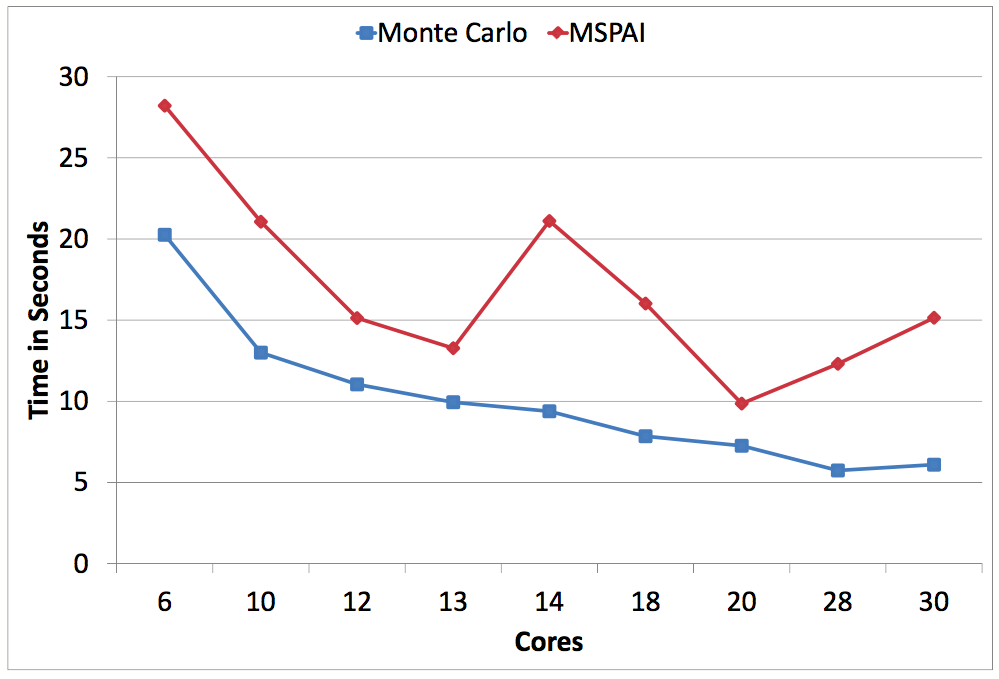
\includegraphics[width=8cm]{img/1}
			\caption[]{Run Times for preconditioning $Psmigr\_3$}
		
		
	\end{figure}
		\begin{figure}[htbp]
		\centering

			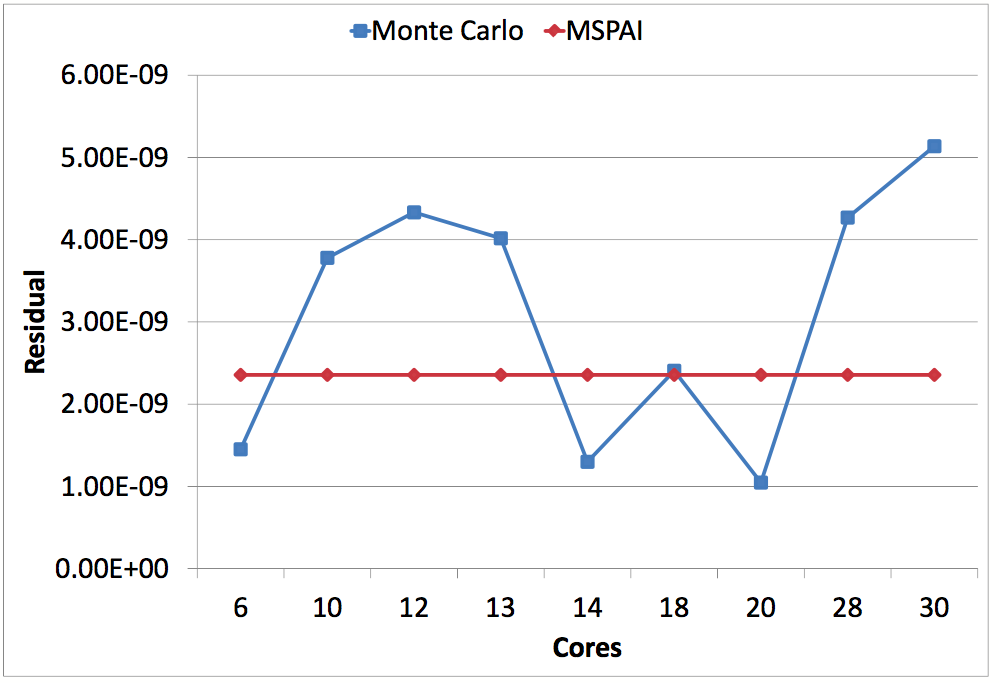
\includegraphics[width=8cm]{img/2}
			\caption[]{Residuals for preconditioning $Psmigr\_3$}
			
	
		
	\end{figure}
			\begin{figure}[htbp]
		\centering
		
		
			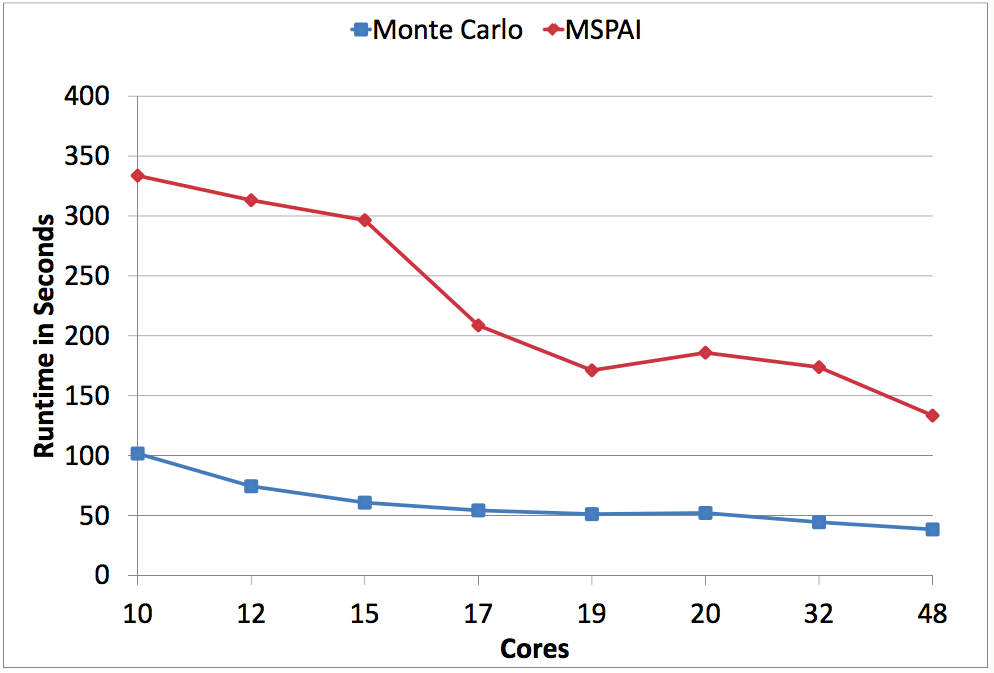
\includegraphics[width=8cm]{img/3}
			\caption[]{Run Times for preconditioning Appu}
		
		
	\end{figure}
		\begin{figure}[htbp]
		\centering
	
		
			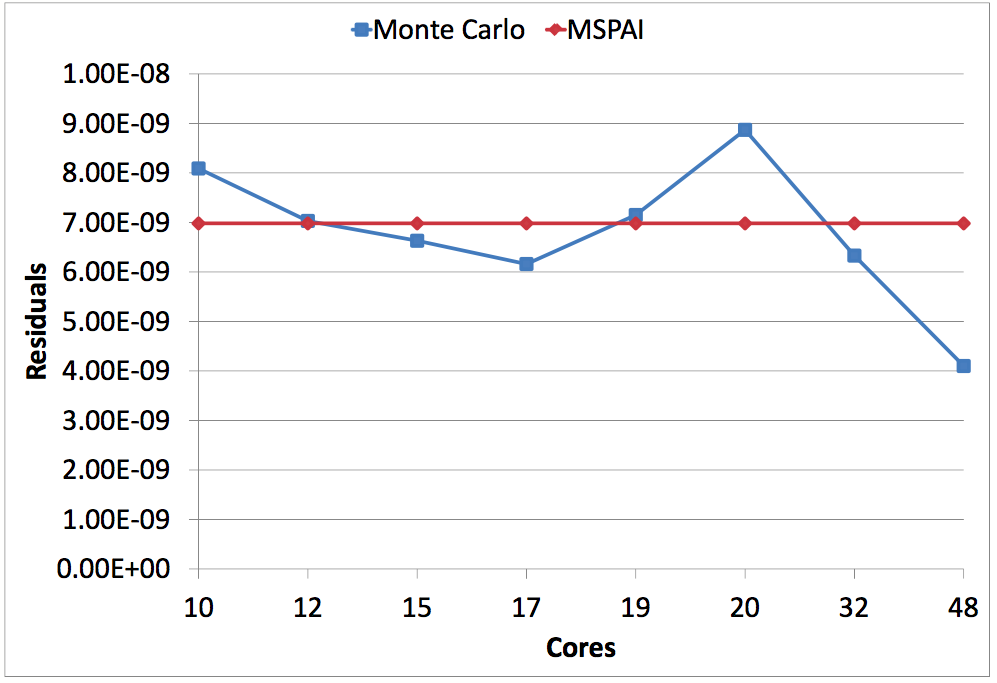
\includegraphics[width=8cm]{img/4}
			\caption[]{Residuals for preconditioning Appu}
		
		
	\end{figure}
	\\\\
2. Evaluation\\
The obtained values for the residuals are quite different between two compared approaches. The MSPAI based deterministic algorithm produces the same result for all runs whereas the Monte Carlo approach, due to its stochastic nature, generates unique preconditioners of a varying quality within the same preconfigured range every time they are recomputed. This is easy to understand, the MCMC method is randomized, so the performance is different every time it runs.\\
From the results it can be seen that our proposed stochastic Monte Carlo approach is able to generate preconditioners of a good quality and within the same margin of error as the deterministic approach taken by MSPAI.\\
When comparing the time needed to compute a preconditioner it is noticeable in the case of $Psmigr\_3$ that both algorithms follow roughly the same scaling pattern. The Monte Carlo approach is significantly faster in computing, especially in the case of fewer processors used.\\
When considering the larger test case of the $Appu$ matrix, the Monte Carlo algorithm outperforms the MSPAI approach quite significantly. It means the MC method has a obvious advantage when the matrix grows larger.\\
\subsection{Conclusion}
The algorithm the arthor propose is able to generate good quality preconditioners by generating a rough inverse using Markov Chain Monte Carlo methods. With an increased size of the input data, handling this information in the main memory of a computer will be a challenge, but with the inherent parallelism in Monte Carlo methods in mind, a parallel data replication approach for even larger matrices is worth investigating.\\
We think a random algorithm like MCMC is suitable and efficient for these kind of problems. We don't need to get a totally accurate solution, the goal is just to roughly estimate a value, the speed is the thing we follow with interest.

\section{Application2: Finding minimum node separators: A Markov chain Monte Carlo method}
\subsection{Introduction}

In networked systems such as communication networks or power grids, graph
separation from node failures can damage the overall operation severely. One
of the most important goals of network attackers is thus to separate nodes so
that the sizes of connected components become small.

 In this work, we consider the problem of finding a minimum $\alpha$-separator, that partitions the graph into connected components of sizes at most n,where n is the number of nodes

\subsection{related work}

the author classify previous work into several categories and summarize them as three parts:\\

1.Network vulnerability and reliability

there is a famous paper by Paolo et al. analyzing the size of the largest component after node removals and the ability to resist filures depending on the type of attacks.Other studies conclude providing a quantitative assessment of how failures affect the network structure.We won't give more details on their work since it is kind of irrelevant to our subject here. \\

2.Deterministic approaches and inapproximability of the $\alpha$ -separator
problem

some studies have developed some polynomial-time algorithms for special topologies(trees and cycles).For example,Shen et al.
also developed polynomial-time dynamic programming algorithms on
tree structures and series-parallel graphs.Nevertheless, we still know little of general topologies.\\

3.Related problems of $\alpha$-separator problem

the $\alpha$-separator problem is a more generalized
version of minimum vertex cover problem($\alpha = 1/n$) and minimum dissociation set problem($\alpha = 2/n$).
Therefore,it's significant to develop an algorithm trying to solve $\alpha$-separator problem.

\subsection{System model}

The author makes following notation and denotation to represent his model.
Consider a simple graph G = (V, E) with V = n. Denote
N (v) as a set of neighbors of a node $v\in V$. The author assumes that the attack
cost is homogeneous across nodes. An $\alpha$-separator W for $1/n\leq\alpha<1$ is defined as a subset of nodes satisfing that the sizes of all components in the graph $G \backslash W$ is equal to or small than $\alpha$n.The author calls this an $\alpha$-separating condition.
$G\backslash W = (V\backslash W, E (V\backslash W)) $is obtained after removing the nodes in W and
all their incident edges, where $ E (V\backslash W) = \{(i, j) \in E| i \in V\backslash W ,j \in V\backslash W \}.$

Here give the definition of $\alpha$-sepatator problem for $1/n\leq \alpha < 1 $ to find a minimum $\alpha$-separator as follows:
$$\min\limits_{W\subseteq V}|W| \mbox{ subject to }f(G \
\ W) \leq \alpha n$$ 
 $$f(G) : \mbox{the size of the largest } \\
 \mbox{connected component in G. }$$
Make a notation $ m = \lfloor \alpha n \rfloor$.
We can prove that there is a polynomial reduction from minimum vertex cover problem to the $\alpha$-separator problem,which means $\alpha$-separator problem is NP-hard.The proof is as follows(the proof is given by [6]):


Construction:

denote: G = (V, E) is the graph we seeks to find a minimum vertex cover. 

Build a new graph $G\textquoteright= (V\textquoteright, E \textquoteright)$ by m
duplications of each vertex $v\in V$. Replace all vertices $v\in V$ with m
vertices $v_1,\cdots,v_m $.  $(v_i, v_j) \in E \textquoteright $ for all $1 \leq i$, $j\leq m$ and $(u_i, v_j) \in E \textquoteright$ for all
$1 \leq i, j \leq m$ when $(u, v) \in E$ for  $u,v \in V$. 

A minimum vertex cover $S\subseteq V$
directly leads to an $\alpha$-separator that contains m duplicate vertices of
each vertex of S. For a minimum $\alpha$-separator of $G\textquoteright$, there is at
least one $u_l$ that belongs to the $\alpha$ -separator if two adjacent
vertices $u_i$ and $v_j$ belong to the same connected component. Otherwise, the size of the
connected component will be strictly greater than m, because all m
duplicate copies of u and $v_j$ are connected. By deleting $v_j$ and adding $u_l$,
we get a new minimum $\alpha$-separator. By repeating this process, we can
obtain a minimum $\alpha$-separator where each connected component
contains exactly m duplicate vertices of some vertices $v\in V$. We can
form a minimum vertex cover that contains those vertices v in the
minimum $\alpha$-separator. Thus, the size of a minimum $\alpha$-separator is $m|S|$
if and only if G has a vertex cover of size $|S|$. Since the minimum vertex
cover problem is NP-hard, the $\alpha$-separator problem is also NP-hard. 

\subsection{Random walk algorithm}


After introducing some necessary notation and proof , let's talk about the essential part: some algorithms developed by the author of this paper.The first one is Random Walk Algorithm.


this algorithm takes one of three actions in every step:

(1)remove v from the attack set W 

(2) add a vertex v in W

(3) stay at the current state

At the same time the author also applies a data sturcture and a corresponding update mechanism for the convenience of computing the sizes of connected components after each action.


Here is a short description of the algorithm:
This algorithm runs over an underlying Markov chain.The state of the Markov chain represents one $\alpha$-separator.the staionary distribution derived from the Markov chain we designed is as follows:
$$ \pi(W) = \frac{\rho^{|W|}}{Z}$$
$$Z \mbox{ is a normalization constant}$$

Here's the pseudo-code of the random walk algorithm(Fig.5)
\begin{algorithmic}[1]
	\STATE $W = V ; W _ { \min } = W$
	\STATE head(v) $= v , \forall v \in V ;$ cluster $( v ) = \{ v \} , \forall v \in V$
	\FOR {step $= 1$ to numStep}
	\STATE Pick a vertex $v \in V$ uniformly at random
	\IF {$v \in W$}
	\STATE newClusterSize=1+$\sum _ { i \in \cup _ { j \in \mathcal { N } ( v ) \backslash W } } { head } ( j )|cluster(j)|$
	\IF {new Cluster Size $\leq \alpha n$}
	\STATE $W = W \backslash \{ v \} ;$ if $| W | < \left| W _ { min } \right| , W _ { \min } = W$
	\STATE cluster(v)= $\bigcup _ { i \in \cup _ { j \in \mathcal { N } ( v ) \backslash W } } { head } ( j )cluster ( i ) \cup \{ v \}$
	\FOR {$i \in$ cluster $( v )$}
	\STATE head $( i ) = v$
	\ENDFOR
	\ENDIF
	\ELSIF {$v \notin W ,$ with probability $\rho$}
	\STATE $W = W \cup \{ v \}$
	\STATE $\mathrm { head } ( i ) = i$ for $i \in \mathcal { N } ( v ) \backslash W$
	\FOR {$i \in \mathcal { N } ( v ) \backslash W$}
	\IF {head $( i ) = i$}
	\STATE cluster $( i ) \leftarrow  { graph }$ Traverse $( i , G \backslash W )$
	\STATE head $( j ) = i , \forall j \in$ cluster $( i )$
	\ENDIF
	\ENDFOR
	\ENDIF
	\ENDFOR
\end{algorithmic}
\begin{figure}[htbp]
	\centering
	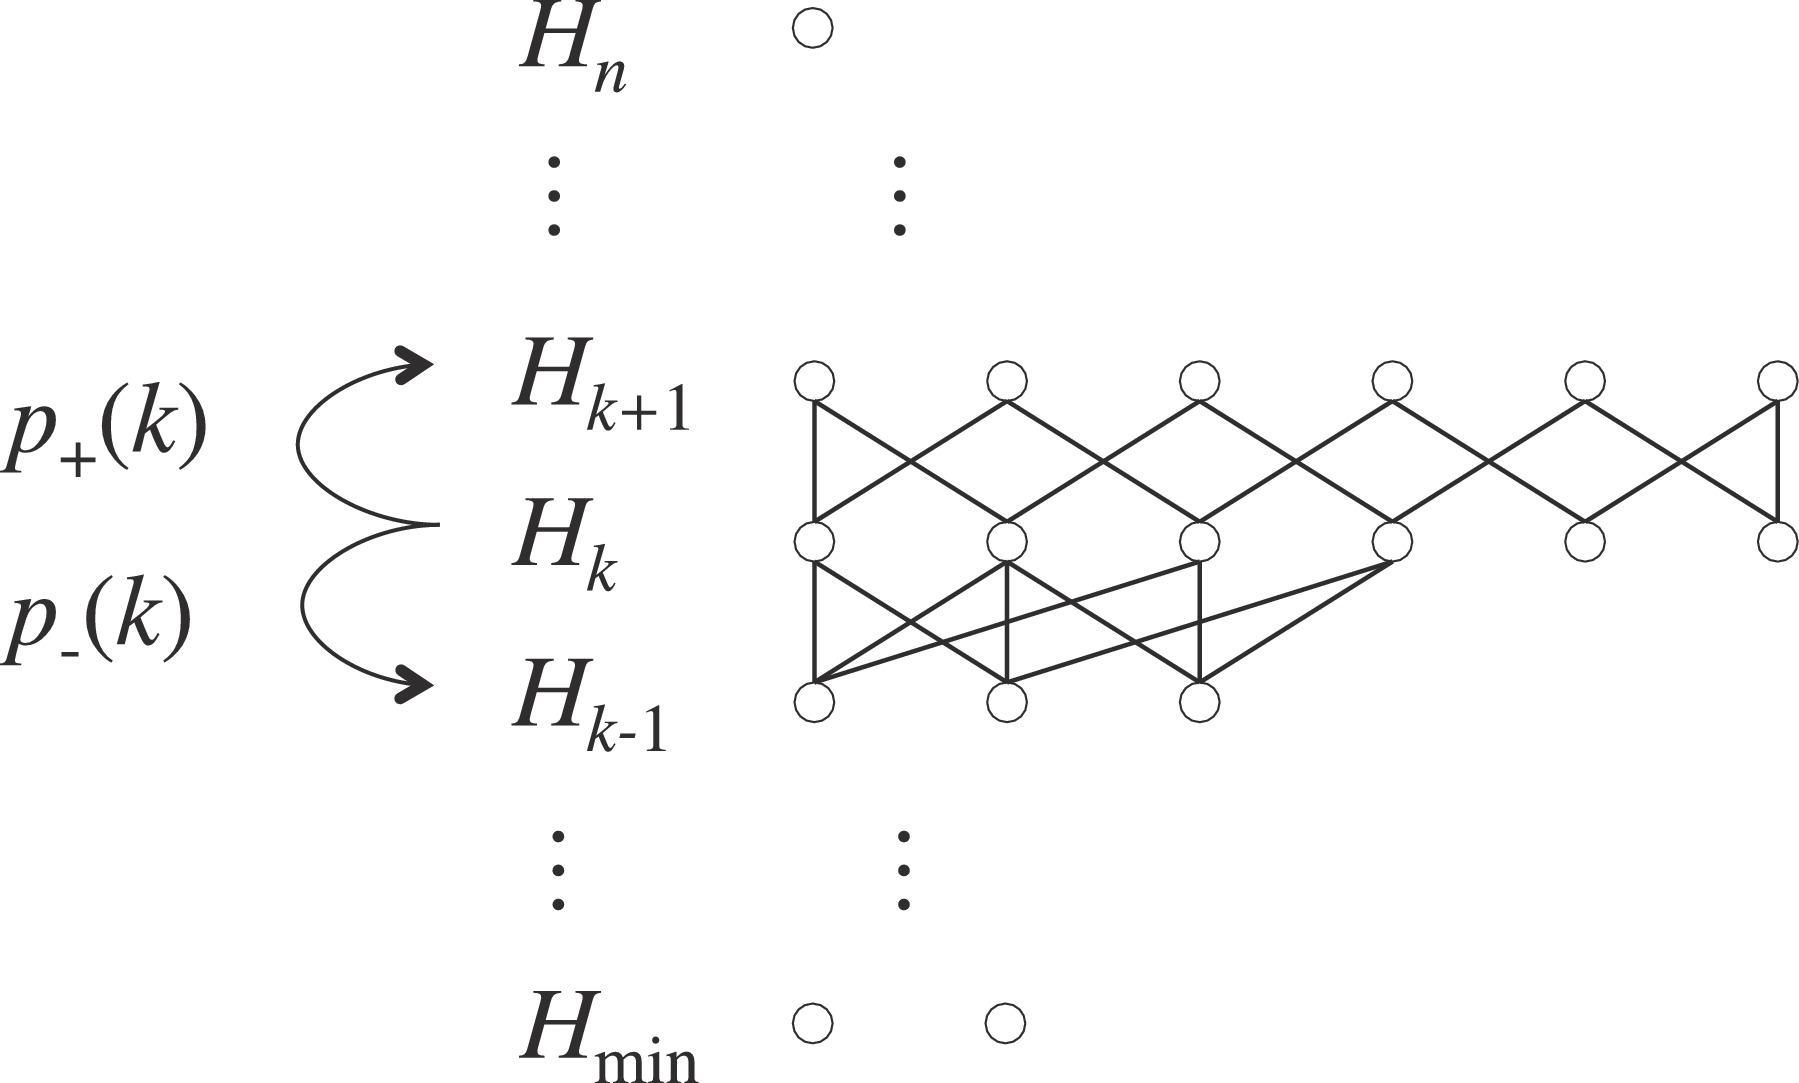
\includegraphics[width=8cm]{img/m}
	\caption[]{Illustration of a hierarchical Markov chain of $\alpha$-separators}
\end{figure}

the following figure(Fig.7) shows how the random walk algorithm workd:

In the beginning,the attact set W includes all vertices,V.$W_{min}$ tracks the $\alpha$-separator which is smallest and has been found.At each step, pick a random vertex $\nu$(in line 4 of the pseudocode)
if\\
(1)$\nu\in W$ 

the algorithm tryies to remove $\nu$ from the attack set W.

 we first compute the size of
the connected component that $\nu$ is associated with. Since this component
is the only one that changes its size, if the size of this component is
less than or equal to $\alpha n$, the vertex addition of $\nu$ is acceptable. When the
new connected component satisfies the condition, a vertex $\nu$ is removed
from W. The vertex $\nu$ is assigned as a head vertex of this component and
the set of associated vertices (i.e., cluster) is updated accordingly.

(2)$\nu\notin W$

the algorithm tries to add $\nu$ in W.

If $\nu\notin W$, the vertex $\nu$ is added to W with probability $\rho$. After $\nu$ is included in
W, the connected component that $\nu$ was associated with can be divided
into multiple components. To track this, we need to traverse from each
neighboring vertex of $\nu$, until all the neighboring vertices are visited
(lines 16–22).
\begin{figure}[htbp]
	\centering
	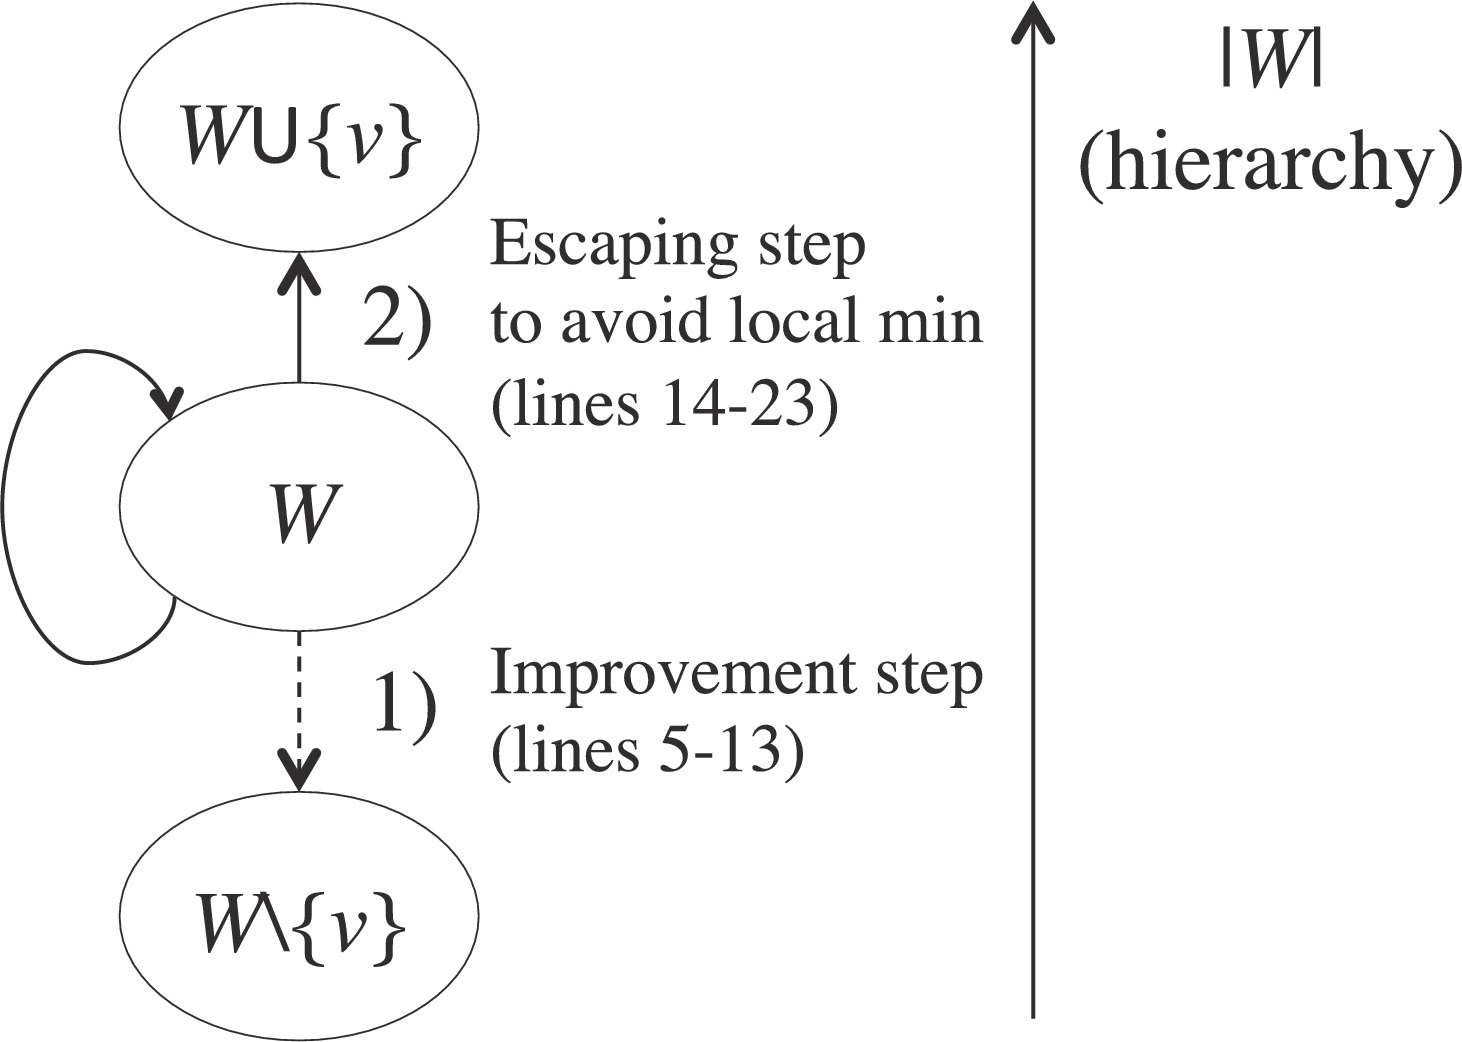
\includegraphics[width=8cm]{img/m2}
	\caption[]{transitions in the algorithm}
\end{figure}


\begin{figure}[htbp]
	\centering
	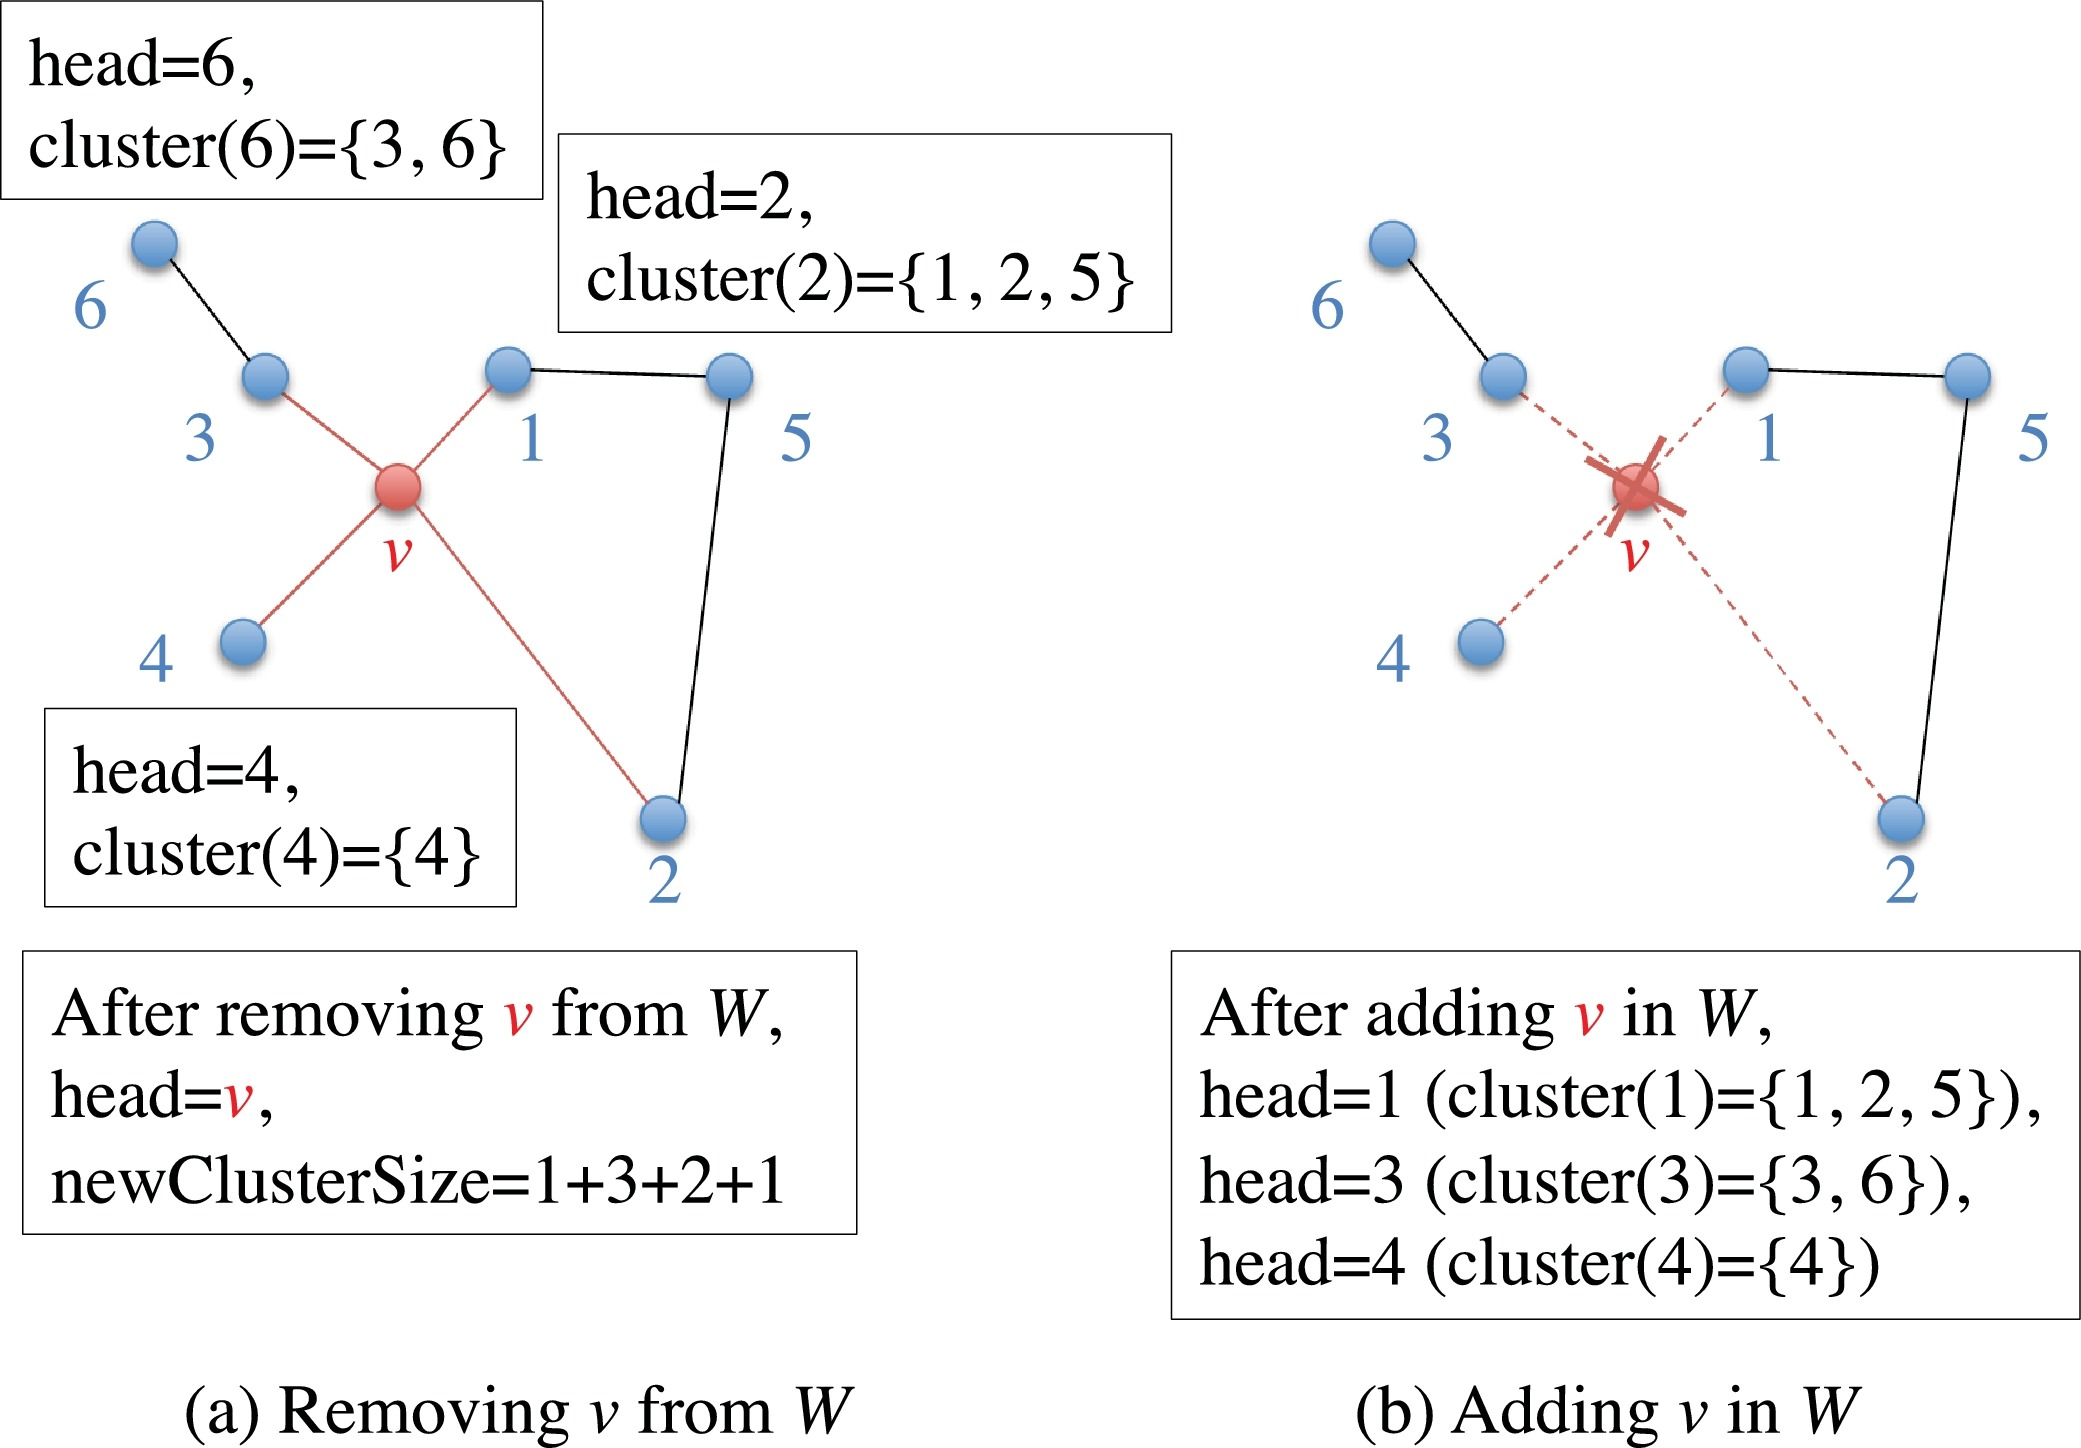
\includegraphics[width=8cm]{img/add_remove}
	\caption[]{An example of vertex removal and addition to W adn updates of heads and clusters}
\end{figure}
 Function graphTraverse$(i, G\backslash W)$ traverses the
graph $G\backslash W$ starting from node i.It will return the connected component
(i.e., cluster) of node i. Pay attention to the fact that if some neighboring nodes are connected
to the node i (e.g., nodes 2 and 1 in Fig. 3 (b)), we will update the head node of
these nodes as i in line 20.
We can use DFS(depth-first search) or BFS(Breadth-first search) to implement it.The complexity of DFS or BFS is $O( V + E )$. The number of graph traversals is
at most the number of neighboring nodes, which is $O(n)$. The complexity
in vertex removal from W is $O(|V|)$ and complexity in vertex
addition to W is $O( V + E )$. 

In conclusion, the overall complexity has relation with the number of steps to run.which means we can not give a fixed complexity.Here's the complexity : $O( |V|^2 + |V||E| )\times numStep$, or $O(n^3)\times numStep$ (numStep : the number of steps to run).


\begin{figure}[htbp]
	\centering
	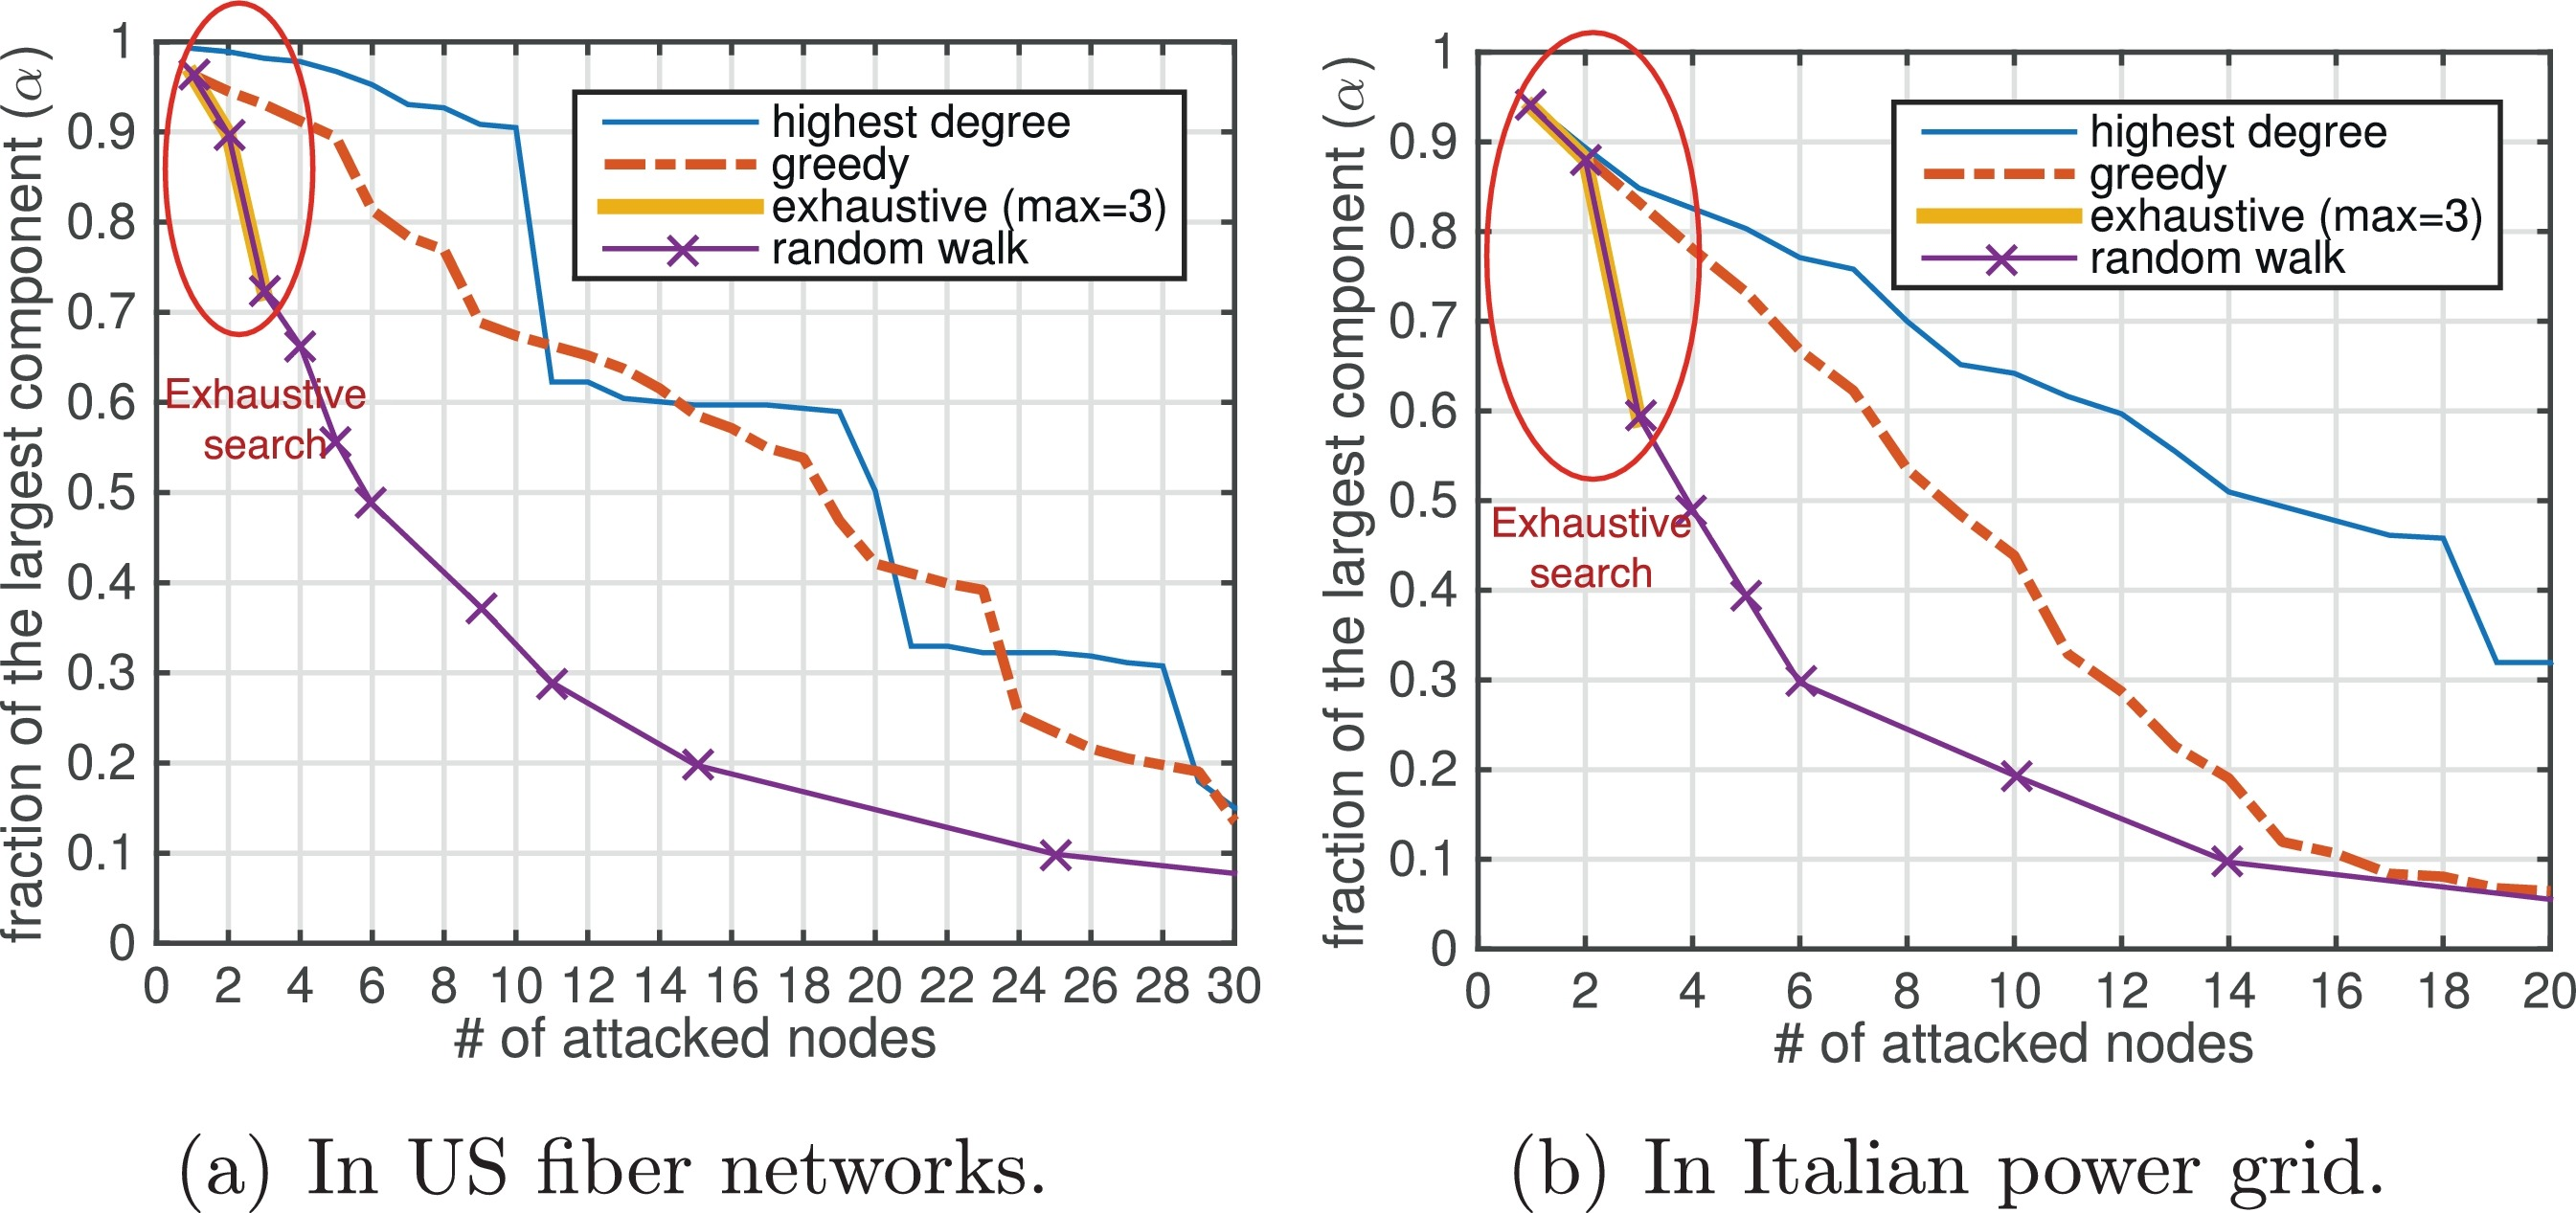
\includegraphics[width=8cm]{img/compresult}
	\caption[]{Comparison with other algorithm}
\end{figure}
\subsection{Simulation results}
\begin{figure*}[htbp]
	\centering 
	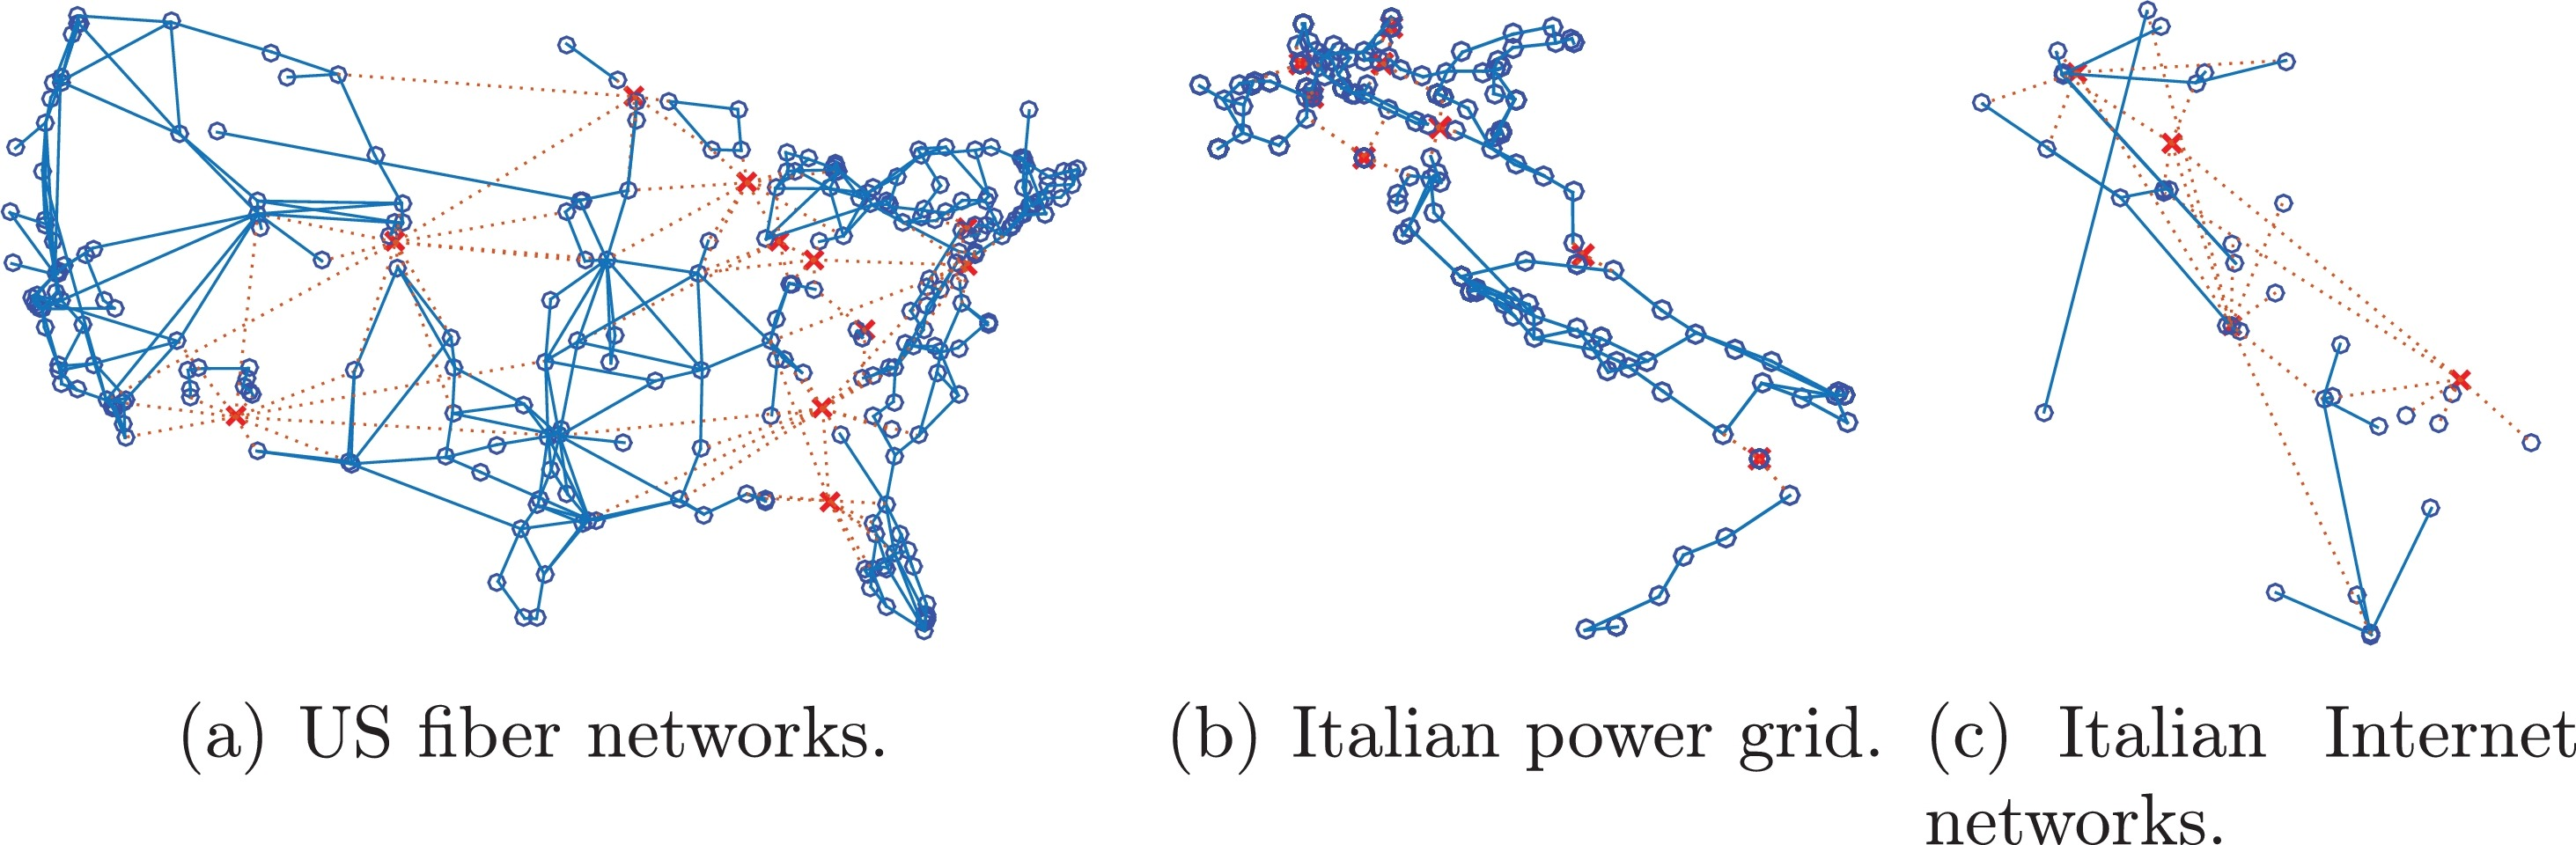
\includegraphics[height=4cm,width=13cm]{img/networks}
	\caption{the networks the author uses }
\end{figure*}



(1)Comparison with other algorithms
In this paper the author compare his algorithm with exhaustive search and two simple heuristic algorithms: greedy and highest-degree-first.
The algorithm is tested on various real and generated topologies:US fiber networks, Italian power grid and Internet network.(Fig.9)

(1)the exhaustive search

it requires computing the sizes of components for each subset, which takes $O(n^3)$
computations. The number of subsets with m nodes is $O(n^m)$. Finding a
minimum takes $O(n^m)$ computations. Thus, the exhaustive search for
subsets with m nodes takes $O(n^{m+3})$ computations. 

(2) highest-degree first algorithm 

short description of this algorithm:Attack vertices are chosen in the order of their node degree, i.e., the number
of neighboring vertices. Break the tie randomly.

In the beginning,it sorts the vertices by their degree which only takes
$O(nlog (n))$ computations. In order to obtain the sizes of the components, highest-degree first algorithm  runs a graph traverse algorithm no more than n times. Therefore , the complexity : $O
(n^3)$. 

(3)greedy algorithm 

short description of this algorithm: In each iteration, for each candidate vertex that is not in W, it computes the size of the largest connected component after adding the vertex. Then, the
vertex with the largest marginal decrease is chosen. Break the tie randomly.

in each iteration, the greedy algorithm sorts the vertices taking $O(n^2log (n))$ computations, but the complexity is still $O(n^3)$ from the graph traverses. 
\\

In conclusion, the highest-degree-first and greedy algorithms perform much better than our algorithm in terms of time complexity(with $O(n^3)$ iterations).But their performance is much worse than our random
walk algorithm in terms of results. The exhaustive search is optimal.However, it takes a really long
time if m is not small.

\section{Conclusion}
From what we discuss above, we can draw conclusions:
\begin{enumerate}
\item
MCMC is a power tool, and it is based on Bayesian statistics. It can be applied to solve a large variety of data analysis problem.

\item As a standard methodology in MCMC, Metropolis Hastings Algorithm is a miraculously simple way to construct a Markov chain with P as its stationary distribution P. Beginning with a provisional Markov chain $C_1$ satisfying only some minimal requirements, it turns out to be very easy to modify $C_1$, making it into another chain $C_2$. 

\item Gibbs sampling is a derivative of Metropolis Hastings Algorithm, which is pretty powerful for related variables.

\item For Metropolis Hastings Algorithm and its derivatives, we usually have a dilemma, for exploration and exploitation. To solve it, we usually use a dynamic epsilon and annealing Algorithm.
\end{enumerate}
% use section* for acknowledgment
\ifCLASSOPTIONcompsoc
  % The Computer Society usually uses the plural form
  \section*{Acknowledgments}
\else
  % regular IEEE prefers the singular form
  \section*{Acknowledgment}
\fi


$[1]$Ziyu Shao

% Can use something like this to put references on a page
% by themselves when using endfloat and the captionsoff option.
\ifCLASSOPTIONcaptionsoff
  \newpage
\fi



\begin{thebibliography}{1}
\bibitem{IEEEhowto:kopka}
Stra$\ss$burg J, Alexandrov V. Enhancing Monte Carlo preconditioning methods for matrix computations[J]. Procedia Computer Science, 2014, 29: 1580-1589. 
\bibitem{IEEEhowto:kopka}
A study of computational complexity of algorithms for numerical methods.University of Rajasthan, 2014.
\bibitem{IEEEhowto:kopka}
T. Barnard, Stephen and Grote, Marcus. (1999). A Block Version of the SPAI Preconditioner. 
\bibitem{IEEEhowto:kopka}
Stra$\ss$burg, Janko, Alexandrov, Vassil. (2013). On scalability behaviour of Monte Carlo sparse approximate inverse for matrix computations. 10.1145/2530268.2530274. 
\bibitem{IEEEhowto:kopka}
Lee J, Kwak J, Lee H W, et al. Finding Minimum Node Separators: A Markov Chain Monte Carlo Method[J]. Reliability Engineering and System Safety, 2018.
\bibitem{IEEEhowto:kopka}
Sidi MAM. K-separator problem, Ph.D. thesis. Evry, Institut National des
Télécommunications; 2014.
\bibitem{IEEEhowto:kopka}
Levin DA, Peres Y, Wilmer EL. Markov chains and mixing times. American
Mathematical Society; 2009.
\end{thebibliography}

% that's all folks
\end{document}


